\documentclass[11pt]{article}
\usepackage{styles} 
\title{Sketch of talk}
\begin{document}
\maketitle
% Most likely -- introduce the background, give intuition for the proof (and sketch some of the other structure results in ANT?). [[Sketch overarching ideas?]]

% Overview: Let $K$ be a fixed number field [finite extension of $\Q$] of degree $[K : \Q] = n = r + 2s$ ($r$ the number of embeddings $K \hookrightarrow \R$, $s$ the number of conjugate pairs of embeddings $K \hookrightarrow \C$) -- Talk a bit about how these embedding numbers are well defined (separability implies $K = \Q(\a)$, and look at $f_\Q^\a \in \Q[x]$)
% \begin{enum}
%     \item \emph{Background:}
%     \begin{enum2}
%         \item Number field objects and constants
%         \begin{enum2}
%             \item Ring of integers [[Integral closure?]]; properties (unique prime ideal factorisation)
%             \item Ideal group (fractional ideals; every ideal is ``invertible''); the ideal norm (reasonable notion of ``size''); ideal class group, the class number (finiteness -- ``every ideal class contains an \underline{integral} ideal of bounded norm'')
%             \item Unit group (structure theorem and regulator)
%             \item Discriminant (description with factorisation -- getting less primes than expected)
%         \end{enum2}
%     \item Dedekind zeta function -- Motivate as a generalisation of Riemann zeta.
%     \end{enum2}
% \end{enum}

Overarching idea: give an example with $K = \Q(i)$, sketching the key ideas behind the proof. Run through an example of computing $\lim_{s \to 1^+} (s - 1)\zeta_{\Q(i)}(s)$. Todo:
\begin{enum}
    \item Introduce the $\zeta_{\Q(i)}(s) = \sum_{0 \neq I \subseteq \Z[i]}\frac1{[\Z[i] : I]^s} = \sum_{a \geq 0, b > 0}\frac1{(a^2 + b^2)^{s/2}}$.
    \item Rewrite $\zeta_{\Q(i)}$ in terms of point counting over a cone in $\C$.
    \item Bring in theorem 3 (in weak generality) and sketch proof.
    \item Compute the volumes $v$ and $\Delta$ (quite straightforward with $\Z[i] \hookrightarrow \Q(i) \hookrightarrow \C$) to show 
    $$
        \lim_{s \to 1^+}(s - 1)\zeta_{\Q(i)}(s) = \frac\pi4
    $$
    \item Talk a little bit about the generalisation -- residues of arbitrary Dedekind zeta functions.
\end{enum}
\section{Introduction}
% The key idea: introduce $\zeta_{\Q(i)}(s)$, reason about convergence for $s > 1$ (hence $\Re(s) > 1$), compute $\Res_{s = 1}\zeta_{\Q(i)}$ [and outline procedure that generalises with some slightly more annoying parts]

For a number field $K$, the analytic class number formula is the residue of the Dedekind zeta function $\zeta_K$ at $s = 1$, and carries fundamental data about the number field, and is closely tied to the distribution of ideals in the associated ring of integers $\o_K \subseteq K$ (which plays a similar role to $\Z \subseteq \Q$). We give the idea for computing this residue in the case $K = \Q(i)$, and briefly discuss the generalisation to arbitrary number fields.

The Dedekind zeta function for $\Q(i)$ is defined by
$$
    \zeta_{\Q(i)}(s) = \sum_{0 \neq I \subseteq \Z[i]} \frac{1}{[\Z[i] : I]^s} 
$$
We note the index of an ideal $I = (a + bi)$ (principal as $\Z[i]$ admits a Euclidean algorithm as every point in $\C$ is within $\sqrt{2}/2$ of one in $\Z[i]$) corresponds to the number of points in the square with corners $(0, 0), (a, b), (a - b, b + a)$ and $(-b, a)$ (i.e. the image of the unit square $[0, 1]^2$ under multiplication by $a + bi$) excluding the sides away from the origin (i.e. $(a, b)$ to $(a - b, b + a)$ and $(a - b, b + a)$ to $(-b, a)$), which we can count by splitting the square as below (which shows the case where $a \geq b$):
\begin{center}
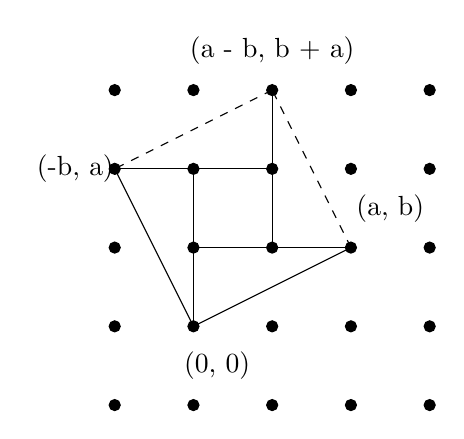
\begin{tikzpicture}
    \draw[fill] (2,1) circle (2pt) coordinate (21);
    \draw[fill] (-1,1) circle (2pt) coordinate (-11);
    \draw[fill] (0,1) circle (2pt) coordinate (01);
    \draw[fill] (1,0) circle (2pt) coordinate (10);
    \draw[fill] (-1,0) circle (2pt) coordinate (-10);
    \draw[fill] (0,-1) circle (2pt) coordinate (0-1);
    \draw[fill] (0,0) circle (2pt) coordinate (00);
    \draw[fill] (-1,2) circle (2pt) coordinate (-12);
    \draw[fill] (-1,-1) circle (2pt) coordinate (-1-1);
    \draw[fill] (-2,-1) circle (2pt) coordinate (-2-1);
    \draw[fill] (1,-1) circle (2pt) coordinate (1-1);
    \draw[fill] (1,-2) circle (2pt) coordinate (1-2);
    \draw[fill] (1,1) circle (2pt) coordinate (11);
    \draw[fill] (2,0) circle (2pt) coordinate (20);
    \draw[fill] (2,-1) circle (2pt) coordinate (2-1);
    \draw[fill] (2,-2) circle (2pt) coordinate (2-2);
    \draw[fill] (-2,0) circle (2pt) coordinate (-20);
    \draw[fill] (-2,1) circle (2pt) coordinate (-21);
    \draw[fill] (-2,2) circle (2pt) coordinate (-22);
    \draw[fill] (0,2) circle (2pt) coordinate (02);
    \draw[fill] (1,2) circle (2pt) coordinate (12);
    \draw[fill] (2,2) circle (2pt) coordinate (22);
    \draw[fill] (0,-2) circle (2pt) coordinate (0-2);
    \draw[fill] (-1,-2) circle (2pt) coordinate (-1-2);
    \draw[fill] (-2,-2) circle (2pt) coordinate (-2-2);
    \node[] at (-0.7, -1.5) {(0, 0)};
    \node[] at (1.5, 0.5) {(a, b)};
    \node[] at (0, 2.5) {(a - b, b + a)};
    \node[] at (-2.5, 1) {(-b, a)};
    \draw[] (-1-1) -- (10);
    \draw[dashed] (10) -- (02);
    \draw[dashed] (02) -- (-21);
    \draw[] (-21) -- (-1-1);
    \draw[] (-1-1) -- (-11);
    \draw[] (-21) -- (01);
    \draw[] (02) -- (00);
    \draw[] (10) -- (-10);
\end{tikzpicture}
\end{center}
where the dashed lines indicate that we do not count point on these lines (including the corners). We can move the top two rectangles down, giving 
\begin{center}
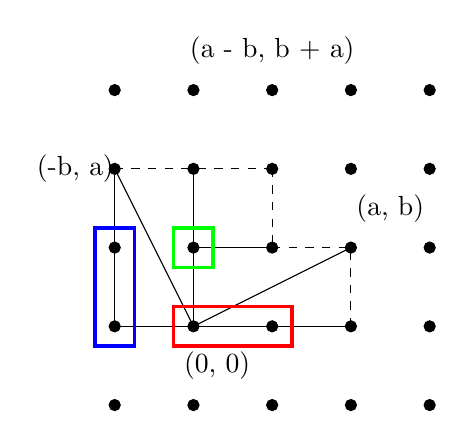
\begin{tikzpicture}
        \draw[fill] (2,1) circle (2pt) coordinate (21);
        \draw[fill] (-1,1) circle (2pt) coordinate (-11);
        \draw[fill] (0,1) circle (2pt) coordinate (01);
        \draw[fill] (1,0) circle (2pt) coordinate (10);
        \draw[fill] (-1,0) circle (2pt) coordinate (-10);
        \draw[fill] (0,-1) circle (2pt) coordinate (0-1);
        \draw[fill] (0,0) circle (2pt) coordinate (00);
        \draw[fill] (-1,2) circle (2pt) coordinate (-12);
        \draw[fill] (-1,-1) circle (2pt) coordinate (-1-1);
        \draw[fill] (-2,-1) circle (2pt) coordinate (-2-1);
        \draw[fill] (1,-1) circle (2pt) coordinate (1-1);
        \draw[fill] (1,-2) circle (2pt) coordinate (1-2);
        \draw[fill] (1,1) circle (2pt) coordinate (11);
        \draw[fill] (2,0) circle (2pt) coordinate (20);
        \draw[fill] (2,-1) circle (2pt) coordinate (2-1);
        \draw[fill] (2,-2) circle (2pt) coordinate (2-2);
        \draw[fill] (-2,0) circle (2pt) coordinate (-20);
        \draw[fill] (-2,1) circle (2pt) coordinate (-21);
        \draw[fill] (-2,2) circle (2pt) coordinate (-22);
        \draw[fill] (0,2) circle (2pt) coordinate (02);
        \draw[fill] (1,2) circle (2pt) coordinate (12);
        \draw[fill] (2,2) circle (2pt) coordinate (22);
        \draw[fill] (0,-2) circle (2pt) coordinate (0-2);
        \draw[fill] (-1,-2) circle (2pt) coordinate (-1-2);
        \draw[fill] (-2,-2) circle (2pt) coordinate (-2-2);
        \node[] at (-0.7, -1.5) {(0, 0)};
        \node[] at (1.5, 0.5) {(a, b)};
        \node[] at (0, 2.5) {(a - b, b + a)};
        \node[] at (-2.5, 1) {(-b, a)};
        \draw[] (-1-1) -- (10);
        \draw[] (-21) -- (-1-1);
        \draw[] (-1-1) -- (-11);
        \draw[dashed] (-21) -- (01);
        \draw[dashed] (01) -- (00);
        \draw[] (-10) -- (00);
        \draw[dashed] (00) -- (10);
        \draw[] (-2-1) -- (-21);
        \draw[] (-2-1) -- (1-1);
        \draw[dashed] (1-1) -- (10);
        \draw[blue, very thick] (-2.25, -1.25) rectangle (-1.75, 0.25);
        \draw[red, very thick] (-1.25, -1.25) rectangle (0.25, -0.75);
        \draw[green, very thick] (-1.25, -0.25) rectangle (-0.75, 0.25);
\end{tikzpicture}
\end{center}
The blue and green rectangles in general each have $ab$ points, while the red rectangle will have $\abs{b - a}^2$ points, giving a total of $\abs{b - a}^2 + 2ab = a^2 + b^2$ points, and so $[\Z : (a + bi)] = a^2 + b^2$ (here $a = 2$, $b = 1$). Our zeta function is thus
$$
    \zeta_{\Q(i)}(s) = \sum_{a \geq 0, b > 0}\frac{1}{(a^2 + b^2)^s}
$$
where we have used the fact that every ideal has a unique generator in the cone $a \geq 0, b > 0$. 

\section{Point-counting}
To show that $\zeta_{\Q(i)}(s)$ is defined for $s > 1$ (and hence $\Re(s) > 1$) and determine $\lim_{s \to 1^+}\zeta_{\Q(i)}(s)$, we can now view $\zeta_{\Q(i)}$ in terms of point-counting, namely as the sum of norms of Gaussian integers in the upper-right quarter plane, and we look to bound these in terms of the Riemann zeta function. Let $X = \set{a + bi \in \C \mid a \geq 0, b > 0}$ be the corresponding upper-right quarter plane. Then 
$$
    \zeta_{\Q(i)}(s) = \sum_{x \in X \cap \Z[i]} \frac1{\abs{x}^{2s}}
$$
and looking at the set $T = X \cap \ol{B_1(0)}$ (which is the upper-right quarter circle), we look to count the number of points $N(r)$ in $rT \cap \Z[i]$ (which is the same as that of $T \cap \frac1r\Z[i]$).

Considering $T \cap \frac1r\Z[i]$, the ratio $N(r)/r^2$ gives the proportion of points in the upper-right unit square part of the lattice $\frac1r\Z[i] \cap [0, 1]^2$ in the set $T$, which will tend towards $\frac\pi4$ (the volume of the upper-right quarter-circle). 

Viewing $N(r)$ instead as the number of points in $rT \cap \Z[i]$, ordering the points $(x_n)_{n \in \N}$ of $X \cap \Z[i]$ in increasing length, we have that $x_1, \ldots, x_n \in \abs{x_n}T$ but $x_n \not\in (\abs{x_n} - \e)T$ for any $\e > 0$. This shows that $N(\abs{x_n} - \e) < n \leq N(\abs{x_n})$, so
$$
    \frac{N(\abs{x_n} - \e)}{(\abs{x_n} - \e)^2}\frac{(\abs{x_n} - \e)^2}{\abs{x_n}^2} < \frac n{\abs{x_n}^2} \leq \frac{N(\abs{x_n})}{\abs{x_n}^2}
$$
and taking $n \to \infty$ (hence $\abs{x_n} \to \infty$) yields $\frac{n}{\abs{x_n}^2} \to \frac\pi4$ by the squeeze theorem. This shows by the comparison test (with the Riemann zeta function) that $\zeta_{\Q(i)}$ converges for $\Re(s) > 1$. We note now that $\lim_{s \to 1^+} (s - 1)\zeta(s) = 1$ since for $s > 1$ we have
$$
    \frac1{s - 1} = \int_1^\infty \frac1{x^s}dx < \sum_{n = 1}^\infty \frac1{n^s} < 1 + \int_1^\infty \frac1{x^s}dx = \frac s{s - 1}
$$
Now for each $\e > 0$, for all sufficiently large $n$ we find 
$$
    \frac1n\brac{\frac\pi4 - \e} < \frac1{\abs{x_n}^2} < \frac1n\brac{\frac\pi4 + \e}
$$
For $s > 1$, taking $s^{\text{th}}$ powers, summing up across sufficiently large $n$ and multiplying by $s - 1$, we find
$$
    \brac{\frac\pi4 - \e}^s(s - 1)\sum_{n > N}\frac1{n^s} < (s - 1)\sum_{n > N}\frac1{\abs{x_n}^{2s}} < \brac{\frac\pi4 + \e}^s(s - 1)\sum_{n > N}\frac1{n^s}
$$
As $s \to 1^+$ the heads of the corresponding sequences are negligible (as they are finite), so we find
$$
    \frac\pi4 - \e \leq \liminf_{s \to 1^+}\sum_{x \in X \cap \Z[i]}\frac1{\abs{x_n}^s} \leq \limsup_{s \to 1^+}\sum_{x \in X \cap \Z[i]}\frac1{\abs{x_n}^s} \leq \frac\pi4 + \e
$$
That is, $\lim_{s \to 1^+} \zeta_{\Q(i)}(s) = \frac\pi4$.
% Rewrite $\zeta_{\Q(i)}$ to rely on point-counting over some cone; introduce this cone informally
\section{Generalisation}
This argument generalises to the Dedekind zeta function $\zeta_K$ of any number field, with some slight caveats. First, point-counting argument given works only for principal ideals. In a general number field, not all ideals of the ring of integers will be principal. However, up to multiplication by a principal ideal there are finitely many classes (and these ideal classes form a finite abelian group in some sense), and so we account for this by splitting the sum by ``ideal class'' applying the argument to each of these, multiplied by an ideal in the ``inverse class'', which will be a sum over principal ideals. The values end up being independent of the ideal class, so this just introduces a term corresponding to the number of ideal classes.

The exact geometric interpretation is also not so simple - in general we view a number field $K$ by embedding it into $n = [K : \Q]$-dimensional space in a way which corresponds to the embeddings $K = \Q(\a) \hookrightarrow \C$ (namely $K_\R \cong \R^r \times \C^s$ where $r$ is the number of real embeddings, $s$ the number of complex embeddings), and the region $X$ we count points on is such that every $x \in K_\R \setminus \set{0}$ splits uniquely as the product of some $x_1 \in X$ and $x_2 \in \o_K^*$ (under this embedding). In general the volume of $X \cap \ol{B_1(0)}$ depends on the density of the (in general infinitely many) units, and the general formula takes the form
$$
    \frac{2^r(2\pi)^s hR}{\omega V}
$$
where $V$ corresponds to the volume of a single grid square in viewing $\o_K$ as a lattice under this geometric interpretation (in our case $\Z[i]$ and the usual unit square of volume 1), $R$ is a term corresponding to the density of units $\o_K^*$ (from $X$), $\omega$ is the number of roots of unity in $K$ and $h$ is the number of ideal classes.
\section{Application or purpose}
Besides being a somewhat nice formula, the analytic class number formula allows for numerical computation of the class number $h$ (which in general is the hardest of these quantities to compute), made slightly easier by the fact that $h$ is necessarily an integer value for each number field $K$. A slightly more general argument relates the distribution of ideals in $\o_K$ of index at most $t$, and by a similar point-counting argument it follows that ideals in $\o_K$ with index at most $t$ are distributed according to $\rho t + O(t^{1 - 1/n})$, where the coefficient $\rho$ of the principal term is exactly this formula (and as a direct consequence, the zeta function extends to $\Re(s) > 1 - 1/n$ except for a simple pole at $s = 1$).
\end{document}